% !TEX root = ./Research_and_SA.tex

\textbf{SIGNIFICANCE}
RNA lies at the center of cellular function. Its most appreciated function is to carry protein blueprints from the genetic code of the nucleus to be manufactured into the protein machines of the cell at the ribosome. Only recently have researchers begun to appreciate its myriad of other functions, many of which also lie at the center of important cellular processes. \comment{X, Y, and Z (maybe the proposed test systems??)} have been recently found to have crucial RNA components.
\comment{More on these systems here. Talk about how localization is important.}
This importance for cellular function necessitates a toolset of probes to study these RNAs as they traverse the cell.
% TODO more here. look at RNA imaging paper intros for examples.

%%%%%%%%%%%%%%%%%%%%%%%%%%%%%%%%%%%%%%%%%%%%%%%%%%%%%%%%%%%%%%%%%%%%%%%%%%%%%%%%
%Riboglow
\begin{wrapfigure}[33]{r}{10cm}
%\vspace{-0.2in}
\begin{centering}
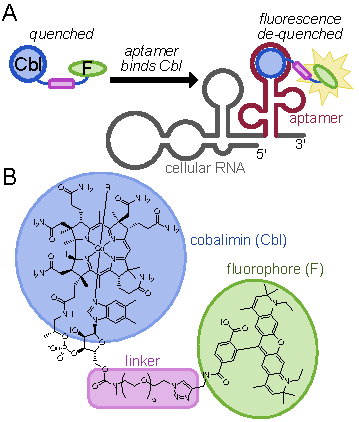
\includegraphics[width=\textwidth]{figures/fig1v2.pdf}

\end{centering}
\footnotesize
\caption{\label{figure:riboglow}
A) Cobalamin acts as a quenching and localization moiety to guide a fluorescent probe to an RNA transcript of interest. When unbound, fluorescence is quenched. In the presence of RNA tagged with the cobalamin aptamer, fluorescence is restored. B) Structure of the generation 1 Riboglow probe. A polyethylene glycol linker of five units (5xPEG) connected to the 5' hydroxly of the cobalamin ribose was used to tether an ATTO 590 fluorophore to the construct.
}
\end{wrapfigure}
%%%%%%%%%%%%%%%%%%%%%%%%%%%%%%%%%%%%%%%%%%%%%%%%%%%%%%%%%%%%%%%%%%%%%%%%%%%%%%%%

\textbf{BACKGROUND}
Proteins benefit from a large imaging toolkit that has been developed over the last \comment{XX} years. Genetically encodable fluorescent proteins are now ubiquitous for the study of the localization of any translated target in the cell. While fluorescent proteins are a mature, well-understood technology, tools for imaging the localization of individual RNA transcripts remain limited. The most popular systems to date include dye-binding aptamers (Spinach\cite{PaigeRNAMimicsGreen2011}, Broccoli\cite{FilonovBroccoliRapidSelection2014}, and Mango\cite{AutourFluorogenicRNAMango2018,DolgosheinaRNAMangoAptamerFluorophore2014}), RNA-binding protein fusions (MS2-FPs), and RNA hybridization probes (RNA FISH).

The most analogous to fluoresecent proteins, dye-binding aptamers utilize exogenously administered dyes that give fluorescence induction upon binding their aptamer.\cite{PaigeRNAMimicsGreen2011,FilonovBroccoliRapidSelection2014,AutourFluorogenicRNAMango2018,DolgosheinaRNAMangoAptamerFluorophore2014} This sequence is encoded \comment{downstream?} of an RNA of interest to track its location in the cell. Though excellent binders for their dyes, the aptamers utilized by this technology are unstable in mammalian cells due to their nonnative structure.\cite{EtzelSyntheticRiboswitchesPlug2017} Additionally, though fluorescence turn-on is excellent \textit{in vitro}, signal induction in cells is low, most likely due to nonspecific binding of the dye.

RNA-binding protein fusions are a much more robust technique for imaging RNA transcripts.\cite{FuscoSinglemRNAMolecules2003} This technique often utilizes the MS2 bacteriophage coat protein that binds a stem loop of RNA. When MS2 is fused to a fluorescent protein, transcripts can be visualized in the cell. In order to concentrate the fluorescence signal above background, multiple stem loops are placed in series (up to 24 in a row). Though this technique has enabled imaging of single transcripts in the cell,\cite{MorisakiRealtimequantificationsingle2016,FuscoSinglemRNAMolecules2003} the resulting protein-RNA complex is prohibitively large for many studies.

\comment{Discuss RNA Fish here??}

Riboglow is a recently developed platform in the Palmer lab that solves many of the drawbacks of the previously discussed techniques (Fig. \ref{figure:riboglow}). The two-component system utilizes a synthetic fluorophore-quencher pair, and a genetically-encoded aptamer. When the construct binds the transcribed aptamer, the fluorophore is dequenched. Like the dye-binding aptamers, Riboglow utilizes a riboswitch receptor domain that natively binds vitamin B\textsubscript{12} (cobalamin, Cbl, Fig. \ref{figure:riboglow}B).\cite{JohnsonJrB12cofactorsdirectly2012} Conveniently, cobalamin is known to act as a fluorescence quencher for a variety of fluorophores.\cite{RosendahlSynthesisbiologicalactivity1982,LeeDesignSynthesisCharacterization2009,SmeltzerSynthesisCharacterizationFluorescent2001} The cobalamin center is conjugated to the fluorophore through a flexible linker that promotes quenching in the unbound state, but enables the fluorophore to reside at a distance in the bound state (Fig. \ref{figure:riboglow}B).

\textbf{APPROACH \underline{Aim 1.} Synthesize improved Riboglow probes.}\\
The main drawback of Riboglow is the poor turn-on that is observed upon probe binding. In this aim, I intend to leverage my background in synthetic chemistry to produce a panel of diverse probe structures that improve fluorescence quenching (and thus signal induction). In previous studies in collaboration with Professor Dorota Gryko (see Gryko letter of support) a small number of linkers and fluorophores were evaluated for quenching and fluorescence turn-on. Linker length and fluorophore wavelength were varied to gauge the quenching ability of cobalamin. Remarkably some degree of quenching occurred in all of the constructs synthesized, regardless of the spectral overlap of the fluorophore and the cobalamin. Intuitively, the largest amount of quenching was observed in the probes with the shortest linkers, and the largest spectral overlap. \textit{To optimize probe function, I will vary linker composition, linker attachment point, and pendant fluorophore.}

%%%%%%%%%%%%%%%%%%%%%%%%%%%%%%%%%%%%%%%%%%%%%%%%%%%%%%%%%%%%%%%%%%%%%%%%%%%%%%%%
%Riboglow
\begin{wrapfigure}[33]{l}{10cm}
%\vspace{-0.2in}
\begin{centering}
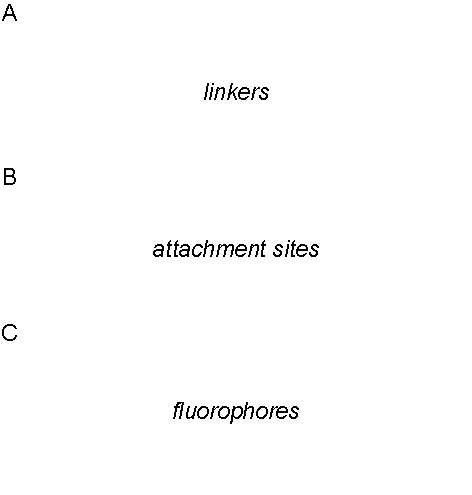
\includegraphics[width=\textwidth]{figures/aim1.pdf}

\end{centering}
\footnotesize
\caption{\label{figure:aim1}
A) Linkers. B) Conjugation sites. C) Fluorophores.
}
\end{wrapfigure}
%%%%%%%%%%%%%%%%%%%%%%%%%%%%%%%%%%%%%%%%%%%%%%%%%%%%%%%%%%%%%%%%%%%%%%%%%%%%%%%%

Ideally, in the unbound state, the cobalamin and the fluorophore would be closely associated to maximize FRET and contact quenching.\cite{LeeDesignSynthesisCharacterization2009} In the RNA-bound state, the molecules would reside at their maximal distance to promote fluorescence. To strike this balance, I propose the use of a synthetic beta turn as the linker between cobalamin and the fluorophore. Such a linker would hold the molecules close in solution, but would be linearized upon binding to the aptamer. A number of such beta turns have been developed. These motifs are as small as twelve amino acids and many are stable to denaturation up to 85 C.\cite{KierProbingLowerSize2008} In the unbound state, such a linker would hold the quencher and fluorophore in close proximity (due to the short distance between the N and C termini of the peptide). When the cobalamin is bound by an aptamer, steric occlusion would force the beta turn to unfold to place the fluorophore-quencher pair at a larger distance. The amino acids of the peptide linker will be varied to adjust the stability of the fold. \comment{More or less specific here? Discuss other linker possibilities?}

Another underexplored variable of the original Riboglow probes is the attachment point for the linker to the cobalamin. Though the 5' hydroxyl of the cobalamin ribose is the most accessible nucleophile on the structure, there exist several other possible sites of conjugation. Perhaps the second most common site is the axial ligand of the cobalt metal itself. Though many studies have taken advantage of the labile nature of certain alkyl modifications at this position,\cite{ShellVitaminB12Tunable2015} others have found alkynyl modifications to be stable to air and light.\cite{ChrominskiReductionfreesynthesisstable2013,RuetzMarkusPhenylethynylcobalaminLightStable2013} Following this precedent, I will synthesize a cobalamin with an alkyne handle attached to the cobalt metal center. Such a molecule has already been synthesized in the lab of Dorota Gryko (see Gryko letter of support), and shown to be amenable to functionalization via dipolar azide-alkyne cycloaddition (AAC).\cite{ChrominskiVitaminB12Derivatives2014} The alkyne handle will be readily conjugated to a variety of linkers with terminal azides. \comment{More detail here??}

%Fluorescence turn-on will also be modulated through changes to the cobalamin metal center. Changes to the electronic environment of the metal center will shift the absorption spectrum, enabling greater spectral overlap with the fluorophore to be quenched.\comment{[Cite]} As the \textit{de novo} synthesis of a molecule such as vitamin B12 would be a massive undertaking,\comment{[Cite]} I will target modifications that can be made through derivatization of the native structure. Without modification of the native ligand, variation of the axial position of cobalamin, and of the metal center itself should be straightforward. There is a large body of work that targets such modifications for the synthesis of so called ``antivitamins".\cite{KrautlerBernhardAntivitaminsB12Structure2015,ChrominskiReductionfreesynthesisstable2013} Through this undertaking, I will be in contact with Professor Dorota Gryko (see Gryko letter of support) one of the experts in this field.

The final variable in the molecular structure of the Riboglow probe is the fluorophore itself. Previous work showed that probes were quenched by the cobalamin center to varying degrees. Quenching correlated somewhat with the spectral overlap of the fluorophore and cobalamin absorption.
% TODO is this 100% true? compare Cy5 excition/emission with ATTO probes.
% TODO make a point here about how redder is better

The new Riboglow probe constructs that I synthesize will be evaluated for brightness in the presence and absence of the cobalamin aptamer.

\textbf{\underline{Aim 2.} Adapt Riboglow for superresolution imaging.}\\
Visualization of the lifecycle of single RNA transcripts as they move throughout the cell remains a holy grail of RNA imaging.\comment{[Cite]} Such a goal should be possible via superresolution imaging and a probe with adequate photostability. Such requirements should be achievable with the Riboglow platform. With a variety of new probe constructs in hand, changes will be made to the cobalamin aptamer to increase fluorescence turn-on. The Palmer lab is a leader in technologies for tool development in mammalian cells.\cite{FiedlerDropletMicrofluidicFlow2017,DeanHighSpeedMultiparameterPhotophysical2015} This expertise will be leveraged for screening libraries of cobalamin aptamers in mammalian cells. Libraries of transcripts will be transduced into mammalian cells, the probe of interest will be administered, and cells will be sorted via flow cytometry.
% QUESTION relative to an FP expression control? or some other RNA-based technique? Broccoli?
% QUESTION what is the absorption of Cbl bound to the riboswitch? does the spectrum change?
In this way, libraries of up to one million members will be screened. Bright variants will be collected, cultured, and resubjected to sorting until the library converges. Sequences will be evaluated through deep sequencing.

%%%%%%%%%%%%%%%%%%%%%%%%%%%%%%%%%%%%%%%%%%%%%%%%%%%%%%%%%%%%%%%%%%%%%%%%%%%%%%%%
%Multicomponent
\begin{wrapfigure}[25]{l}{10cm}
%\vspace{-0.2in}
\begin{centering}
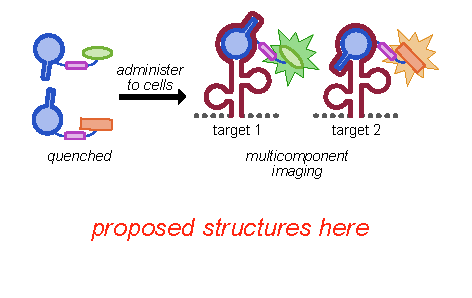
\includegraphics[width=\textwidth]{figures/fig3.pdf}

\end{centering}
\footnotesize
\caption{\label{figure:multicomponent}
A) Mutually orthogonal cobalamin analogs will enable multicomponent RNA imaging. Signal turn-on will only be observed in the presence of the matched pair. B)\comment{Propose some structures.} C) SELEX will be used to screen for aptamers that bind each cobalamin in a mutually-exclusive manner.
}
\end{wrapfigure}
%%%%%%%%%%%%%%%%%%%%%%%%%%%%%%%%%%%%%%%%%%%%%%%%%%%%%%%%%%%%%%%%%%%%%%%%%%%%%%%%

\textbf{\underline{Aim 3.} Develop mutually orthogonal Riboglow probes for multicomponent imaging.}\\
\comment{Don't forget Szostak precedent!\cite{LorschvitroselectionRNA1994}}
% TODO make a point here about how unnatural ligand architectures will help reduce off-target fluorescence.

%%% Local Variables: ***
%%% mode: latex ***
%%% TeX-master: "Research_and_SA.tex" ***
%%% End: ***
